 % -*- root: ../main.tex -*-
\documentclass[../main.tex]{subfiles}
\begin{document}

\chapter{Publications}\label{chap:publications}

\clearpage
\newpage

% ================================================

\section{Mécanismes d'action des récepteurs aux hormones thyroïdiennes durant le développement : Lessons retenues des études sur les amphibiens}\label{sec:bba-review}

\begin{abstract}

Background: Thyroid hormone (TH) receptor (TR) plays critical roles in vertebrate development. However, the in vivo mechanism of TR action remains poorly explored.

Scope of review: Frog metamorphosis is controlled by TH and mimics the postembryonic period in mammals when high levels of TH are also required.
We review here some of the findings on the developmental functions of TH and TR and the associated mechanisms obtained from this model system.

Major conclusion: A dual function model for TR in Anuran development was proposed over a decade ago.
That is, unliganded TR recruits corepressors to TH response genes in premetamorphic tadpoles to repress these genes and prevent premature metamorphic changes.
Subsequently, when TH becomes available, liganded TR recruits coactivators to activate these same genes, leading to metamorphic changes.
Over the years, mo- lecular and genetic approaches have provided strong support for this model.
Specifically, it has been shown that unliganded TR recruits histone deacetylase containing corepressor complexes during larval stages to control metamorphic timing, while liganded TR recruits multiple histone modifying and chromatin remodeling coactivator complexes during metamorphosis.
These complexes can alter chromatin structure via nucleosome position alterations or eviction and histone modifications to contribute to the recruitment of transcriptional machinery and gene activation.

General significance: The molecular mechanisms of TR action in vivo as revealed from studies on amphibian metamorphosis are very likely applicable to mammalian development as well.
These findings provide a new perspective for understanding the diverse effects of TH in normal physiology and diseases caused by TH dysfunction.
This article is part of a Special Issue entitled Thyroid hormone signalling.

\end{abstract}

%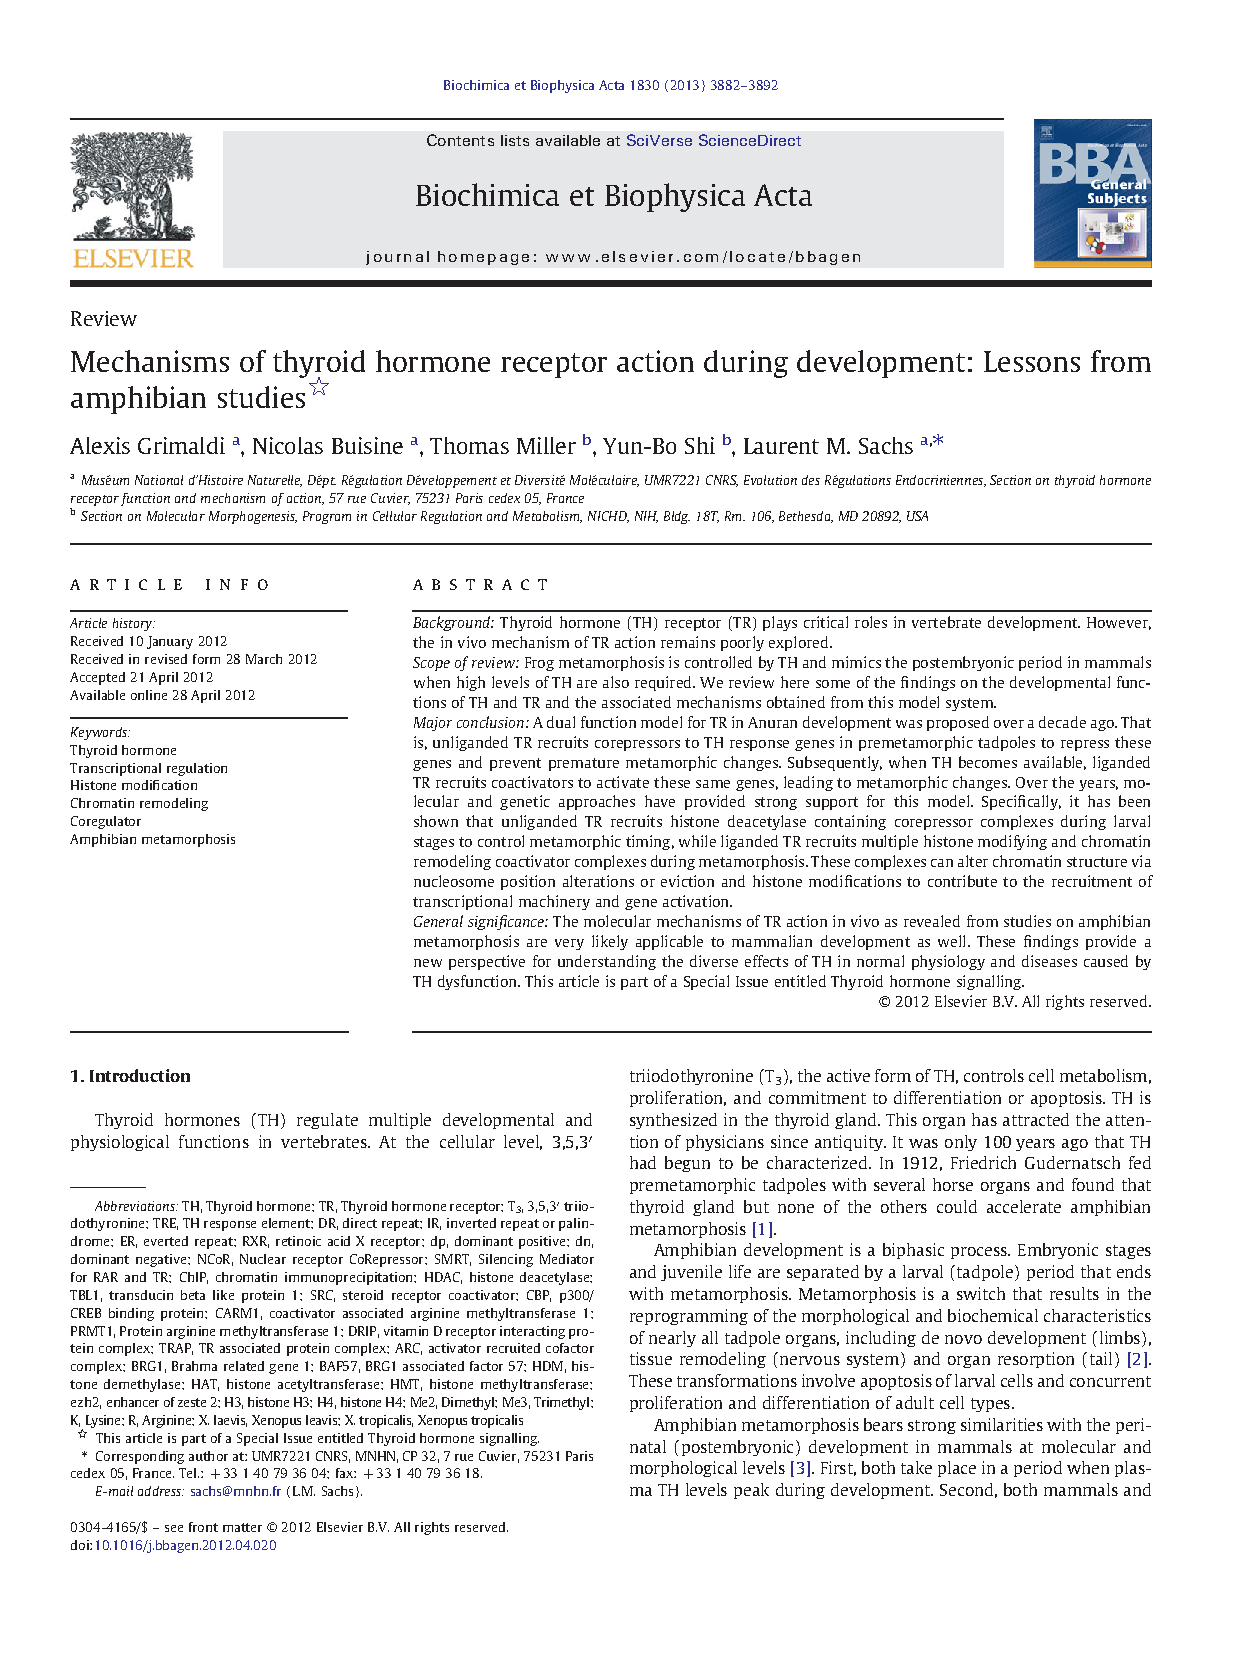
\includepdf[pages={-}]{Publications/bba-review.pdf}

% ====================================================

\clearpage
\newpage

% ====================================================

\section{Les technologies de séquençage à haut débit vont métamorphoser l'analyse de la fonction des récepteurs aux hormones thyroïdiennes pendant le développement de l'amphibien}\label{sec:ctdb-review}

\begin{abstract}

Amphibian metamorphosis is marked by dramatic thyroid hormone (T3)-induced changes including de novo morphogenesis, tissue remodeling, and organ resorption through programmed cell death.
These changes involve cascades of gene regulation initiated by thyroid hormone (TH).
TH functions by regulating gene expression through TH receptors (TR).
TR are DNA-binding transcription factors that belong to the steroid hormone receptor superfamily.
In the absence of ligand, TR can repress gene expression by recruiting a corepressor complex, whereas liganded TR recruits a coactivator complex for gene activation.
Earlier studies have led us to propose a dual function model for TR during development.
In premetamorphic tadpoles, unliganded TR represses transcription involving corepressors.
During metamorphosis, endogenous T3 allows TR to activate gene expression.
To fully understand the diversity of T3 effects during metamorphosis, whole genome analysis of transcriptome and mechanism of TR action should be carried out.
To this end, the new sequencing technologies have dramatically changed how fundamental questions in biology are being addressed and is now making the transition from technology development to being a standard for genomic and functional genomic analysis.
This review focuses on the applications of high-throughput technologies to the field of amphibian metamorphosis.

\end{abstract}

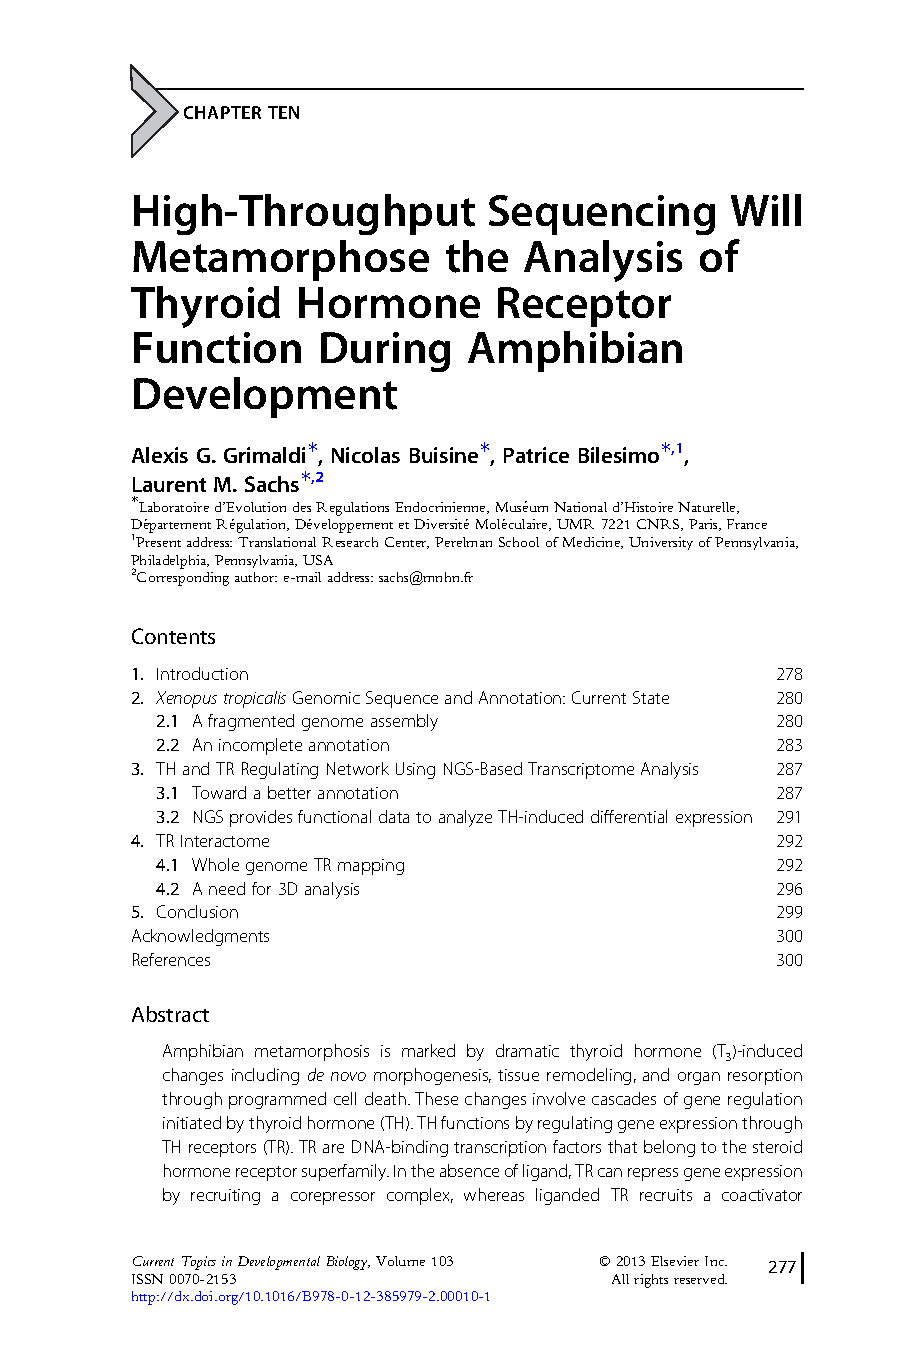
\includepdf[pages={-}]{Publications/ctdb-review.pdf}

\clearpage
\newpage

\section{Re-assembly and re-annotation of the Xenopus tropicalis genome for in vivo ChIA-PET analysis}\label{sec:buisine2014}

\begin{abstract}

Abstract

\end{abstract}

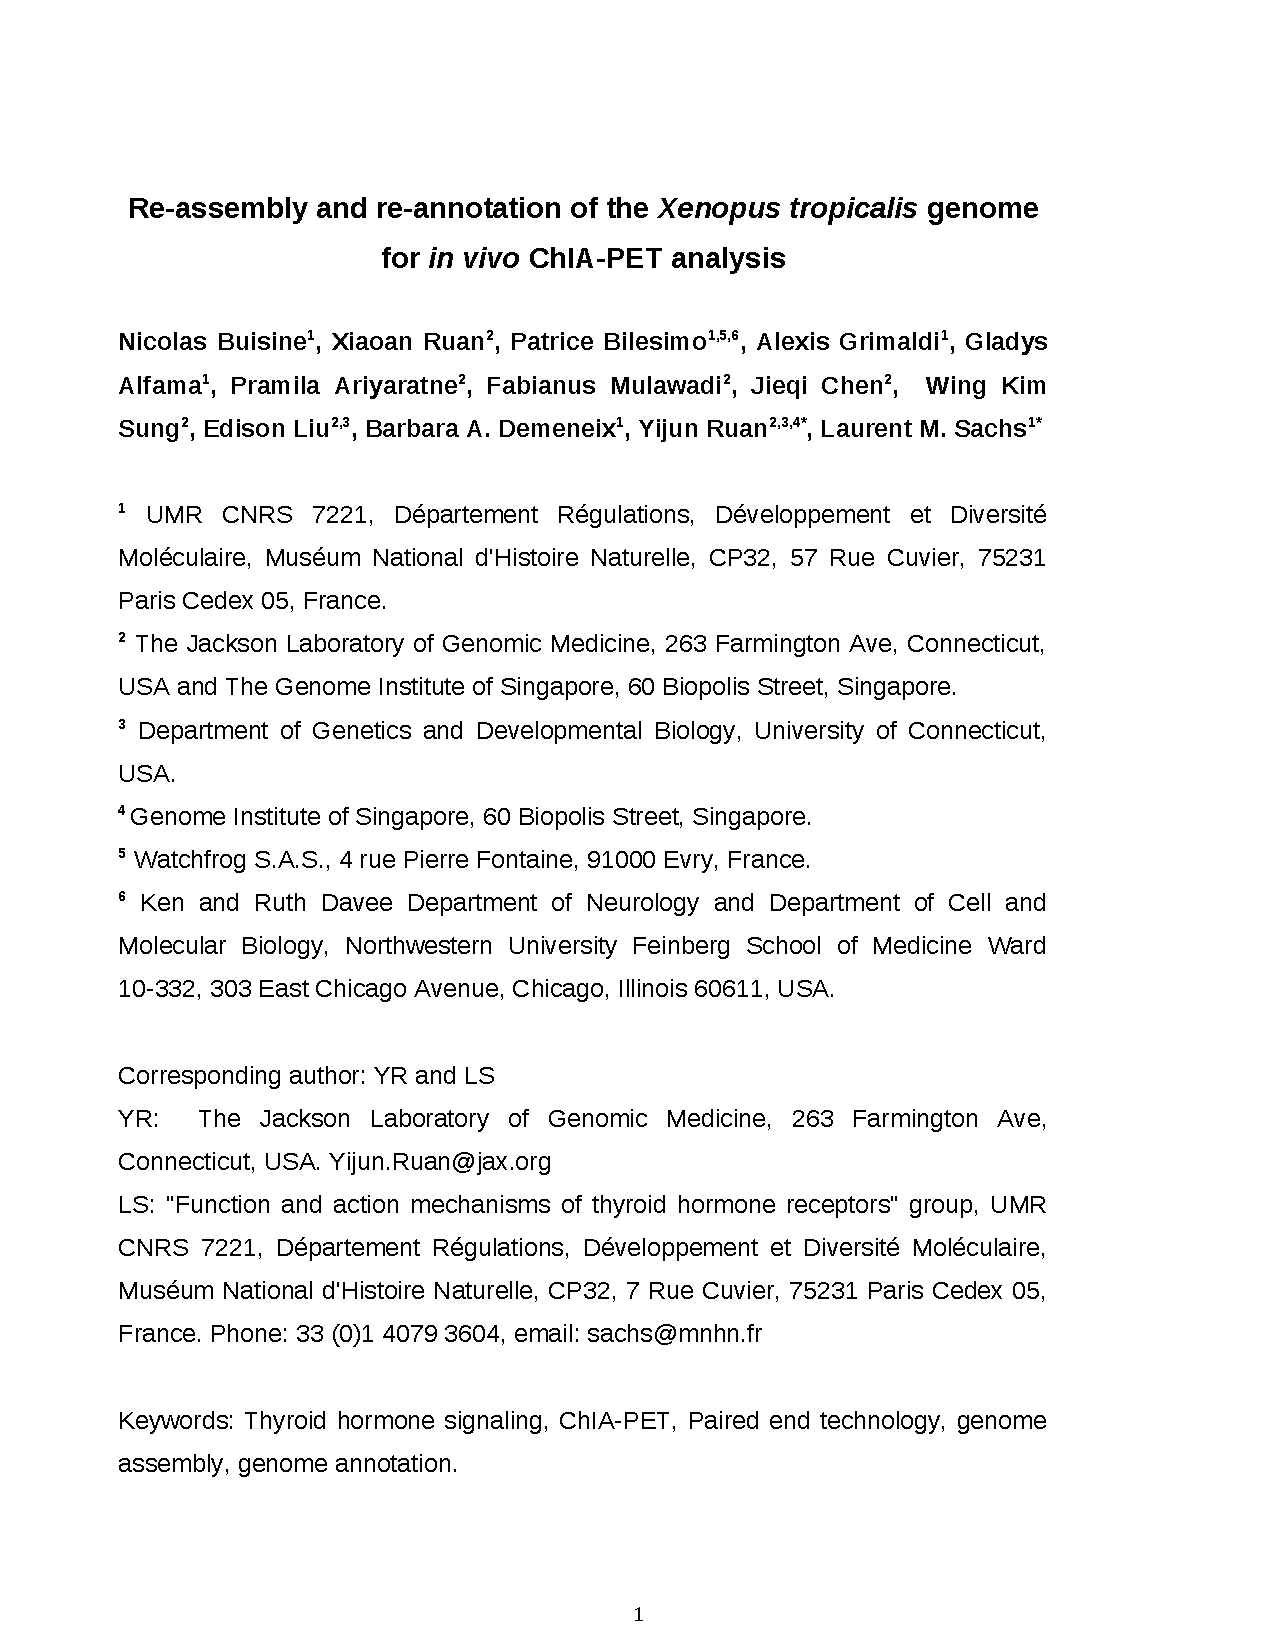
\includepdf[pages={-}]{Publications/buisine2014.pdf}
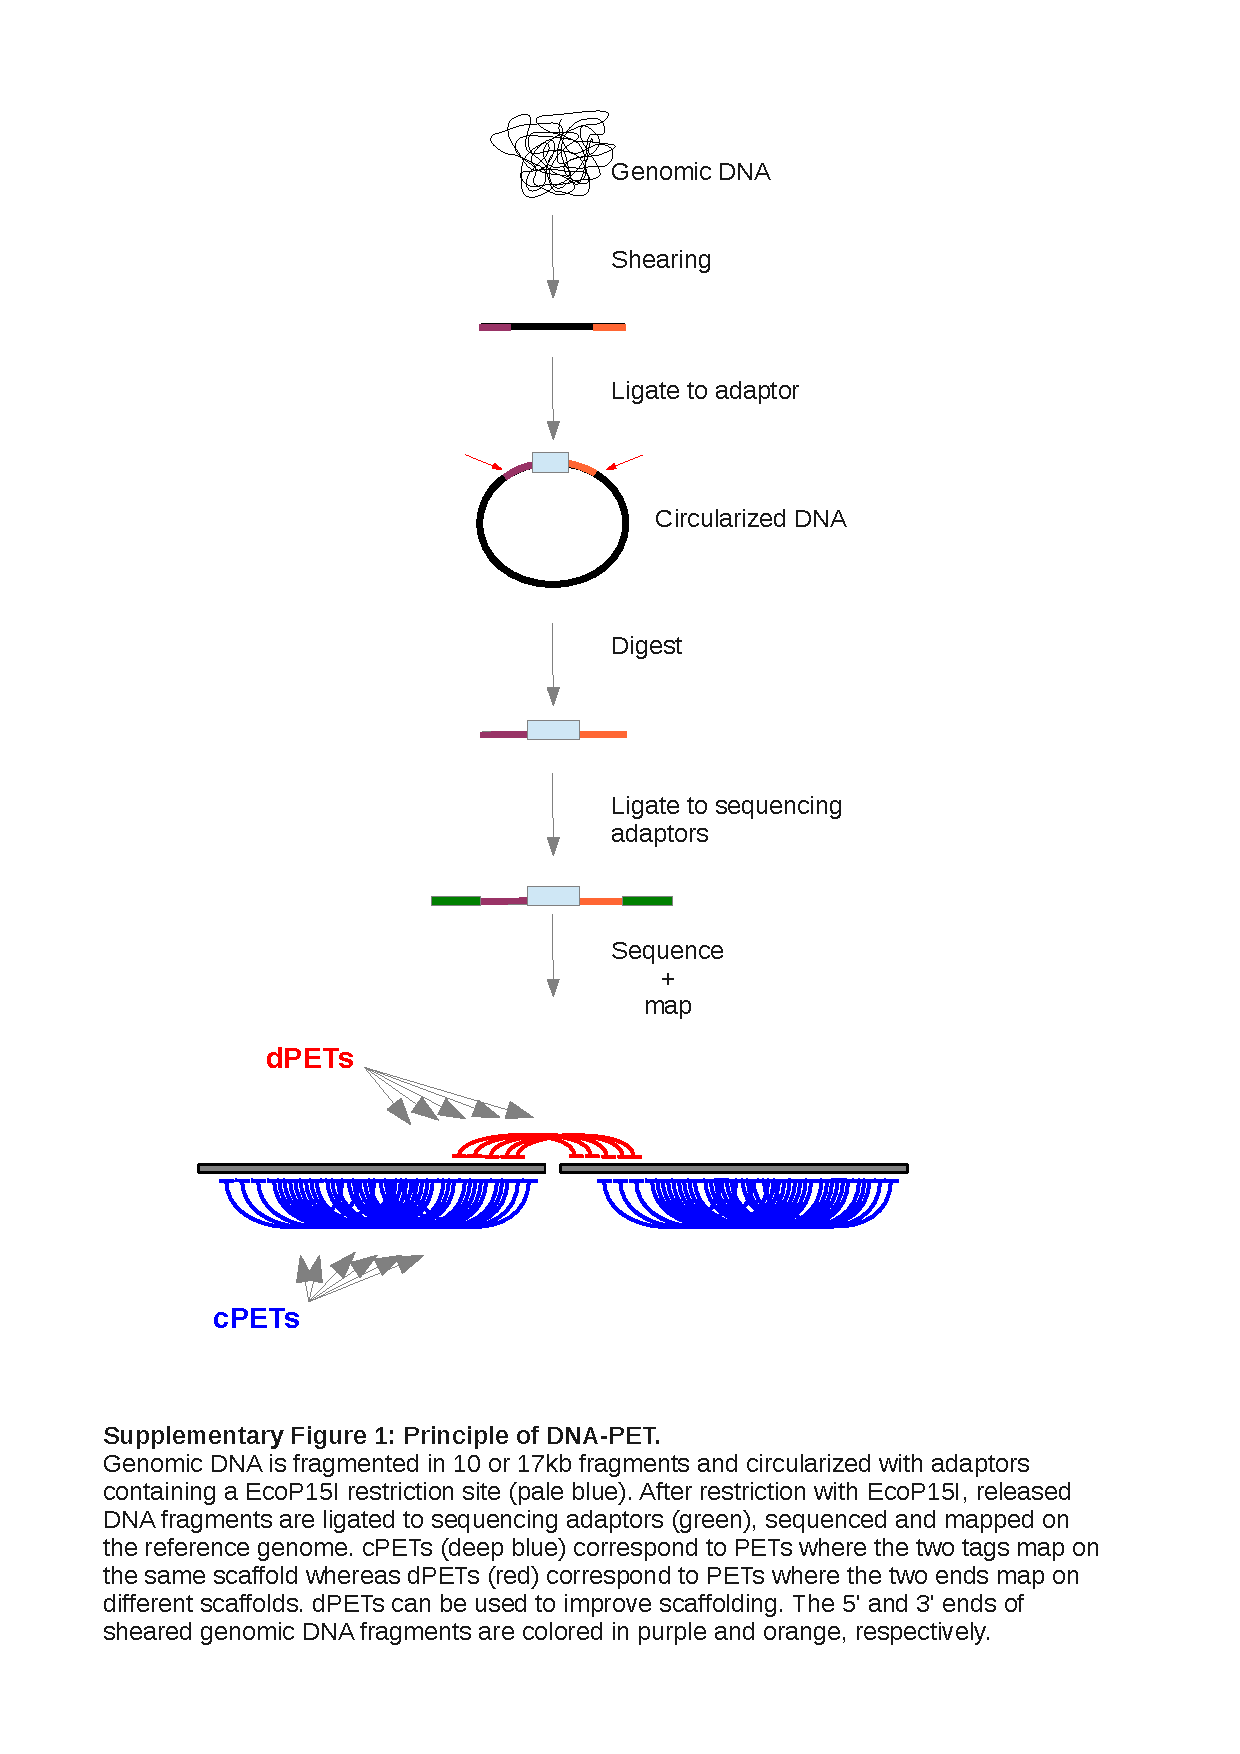
\includepdf[pages={-},nup=1x2,landscape=true]{Publications/buisine2014-sup.pdf}

\end{document}